47. $y=|x-2|+|x+1|=\left[\begin{array}{l}x-2+x+1=2x-1,\ x>2,\\ 2-x+x+1=3,\ x\in[-1;2],\\ -x+2-x-1=-2x+1,\ x<-1.\end{array}\right.$
$$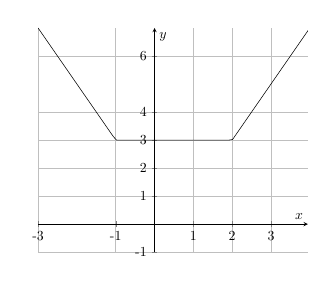
\begin{tikzpicture}[scale=0.5]
\begin{axis}[
    axis lines = middle,
    grid=major,
    legend pos={south west},
    xlabel = {$x$},
    ylabel = {$y$},
    ymin=-1,
    ymax=7,
    xtick={-3,-1,1,3,5,2},
    xticklabels={-3,-1,1,3,5,2},
    ytick={ 6, 2,-6, -2,1,-1,4,-4,3},
    yticklabels={ 6, 2,-6, -2,1,-1,4,-4,3}           ]
	\addplot[domain=-3:5, samples=100, color=black] {abs(x-2)+abs(x+1)};
%\addplot[domain=-3:5, samples=100, color=black] {-abs(x-1)};
%\addplot[domain=-3.1:2.5, samples=100, color=red] {70*abs(1-2*abs(abs(x)-2))-10*x^2+10*x-70};
	%\addlegendentry{$\text{Рис. 1}$};
\end{axis}
\end{tikzpicture}$$
